% Options for packages loaded elsewhere
\PassOptionsToPackage{unicode}{hyperref}
\PassOptionsToPackage{hyphens}{url}
%
\documentclass[
]{article}
\usepackage{amsmath,amssymb}
\usepackage{iftex}
\ifPDFTeX
  \usepackage[T1]{fontenc}
  \usepackage[utf8]{inputenc}
  \usepackage{textcomp} % provide euro and other symbols
\else % if luatex or xetex
  \usepackage{unicode-math} % this also loads fontspec
  \defaultfontfeatures{Scale=MatchLowercase}
  \defaultfontfeatures[\rmfamily]{Ligatures=TeX,Scale=1}
\fi
\usepackage{lmodern}
\ifPDFTeX\else
  % xetex/luatex font selection
\fi
% Use upquote if available, for straight quotes in verbatim environments
\IfFileExists{upquote.sty}{\usepackage{upquote}}{}
\IfFileExists{microtype.sty}{% use microtype if available
  \usepackage[]{microtype}
  \UseMicrotypeSet[protrusion]{basicmath} % disable protrusion for tt fonts
}{}
\makeatletter
\@ifundefined{KOMAClassName}{% if non-KOMA class
  \IfFileExists{parskip.sty}{%
    \usepackage{parskip}
  }{% else
    \setlength{\parindent}{0pt}
    \setlength{\parskip}{6pt plus 2pt minus 1pt}}
}{% if KOMA class
  \KOMAoptions{parskip=half}}
\makeatother
\usepackage{xcolor}
\usepackage[margin=1in]{geometry}
\usepackage{graphicx}
\makeatletter
\def\maxwidth{\ifdim\Gin@nat@width>\linewidth\linewidth\else\Gin@nat@width\fi}
\def\maxheight{\ifdim\Gin@nat@height>\textheight\textheight\else\Gin@nat@height\fi}
\makeatother
% Scale images if necessary, so that they will not overflow the page
% margins by default, and it is still possible to overwrite the defaults
% using explicit options in \includegraphics[width, height, ...]{}
\setkeys{Gin}{width=\maxwidth,height=\maxheight,keepaspectratio}
% Set default figure placement to htbp
\makeatletter
\def\fps@figure{htbp}
\makeatother
\setlength{\emergencystretch}{3em} % prevent overfull lines
\providecommand{\tightlist}{%
  \setlength{\itemsep}{0pt}\setlength{\parskip}{0pt}}
\setcounter{secnumdepth}{-\maxdimen} % remove section numbering
\usepackage[linesnumbered,ruled,vlined]{algorithm2e}
\usepackage{amsmath}
\usepackage{graphicx}
\usepackage{float}
\ifLuaTeX
  \usepackage{selnolig}  % disable illegal ligatures
\fi
\usepackage{bookmark}
\IfFileExists{xurl.sty}{\usepackage{xurl}}{} % add URL line breaks if available
\urlstyle{same}
\hypersetup{
  pdftitle={Cox PH Simulation Algorithm},
  hidelinks,
  pdfcreator={LaTeX via pandoc}}

\title{Cox PH Simulation Algorithm}
\author{}
\date{\vspace{-2.5em}}

\begin{document}
\maketitle

\begin{algorithm}[H]
\caption{Paired Cooker Profile Simulation}
\label{alg:paired-cooker-sim-detail}
\DontPrintSemicolon
\SetKwInOut{Input}{Input}\SetKwInOut{Output}{Output}

\Input{%
  Dataset of observations \(\{(t_i,\{v_k(t_i)\}_{k=1}^K,\mathrm{exp}_i)\}\),\\
  Variable set \(\mathbf V\subseteq\{v_1,\dots,v_K\}\),\\
  Grid size \(n\), matching radius \(\delta\), RNG seed (opt.)
}
\Output{Simulated trajectories \(P^{(1)},P^{(2)}\)}

\BlankLine
\SetKwBlock{Init}{Initialize}{}
\Init{
  set.seed(seed)\;
  ensure \(\mathrm{Td}\in\mathbf V\) and \(\mathrm{exp}\in\mathbf V\)\;
}

\BlankLine
\tcp{\textbf{1.} Normalize and subset}
\If{\(I_{\rm avg}\in\mathbf V\)}{
  \(I_{\rm avg}\leftarrow I_{\rm avg}/\max(I_{\rm avg})\)
}
\(\mathcal S\gets\) rows with no NA in \(\mathbf V\cup\{t\}\)\;

\BlankLine
\tcp{\textbf{2.} Define time grid}
\[
  u_j = \min_i t_i + \frac{j-1}{n-1}\bigl(\max_i t_i - \min_i t_i\bigr),
  \quad j=1,\dots,n
\]

\BlankLine
\tcp{\textbf{3.} Smooth profiles per day}
\ForEach{day \(d\)}{
  \ForEach{variable \(v\in\mathbf V\)}{
    \[
      \hat v_d(u_j)=
      \begin{cases}
        \mathrm{spline}\bigl(\{t_i\}_d,\{v(t_i)\}_d,u_j\bigr),
        &|\{t_i\}_d|>2,\\
        \overline{v}_d,&\text{otherwise.}
      \end{cases}
    \]
  }
}

\BlankLine
\tcp{\textbf{4.} Compute \& center residuals}
\[
  \epsilon_{i,k}=v_k(t_i)-\hat v_{d(i),k}(t_i),\quad
  \epsilon_{i,k}\leftarrow \epsilon_{i,k}-\frac1N\sum_{i}\epsilon_{i,k}
\]

\BlankLine
\tcp{\textbf{5.} Sample two base days}
Draw \(d_1,d_2\sim\mathrm{Uniform}(\{\text{days}\})\)\;

\BlankLine
\tcp{\textbf{6.} Add residuals by experiment}
\For{\(c\in\{1,2\}\)}{
  \(d\leftarrow d_c\)\;
  \For{\(j=1,\dots,n\)}{
    \ForEach{\(v\in\mathbf V\)}{
      let \(R=\{\epsilon_{i,k}:|t_i-u_j|<\delta,\,\mathrm{exp}_i=d\}\) (or all \(\epsilon_{\cdot,k}\) if empty)\;
      \[
        v_k^{(c)}(u_j)=\hat v_d(u_j)+\mathrm{sample}(R)
      \]
    }
  }
}

\BlankLine
\tcp{\textbf{7.} Clamp wind}
If \(\text{Wind}\in\mathbf V\), clamp \(v^{(c)}_{\rm Wind}(u_j)\in[0,2.5]\)\;

\BlankLine
\tcp{\textbf{8.} Combine \& label}
Form \(P^{(c)}=\{(u_j,\{v_k^{(c)}(u_j)\}_k)\}\);  
add label Cooker\,\(=c\)\;

\BlankLine
\tcp{\textbf{9.} Quantile‐map marginals}
For each \(v\), reorder \(\{v_k^{(c)}(u_j)\}\) to match the empirical distribution of \(\{v_k(t_i)\}\)\;

\Return \(\{P^{(1)},P^{(2)}\}\)
\end{algorithm}

\begin{figure}[H]
  \centering
  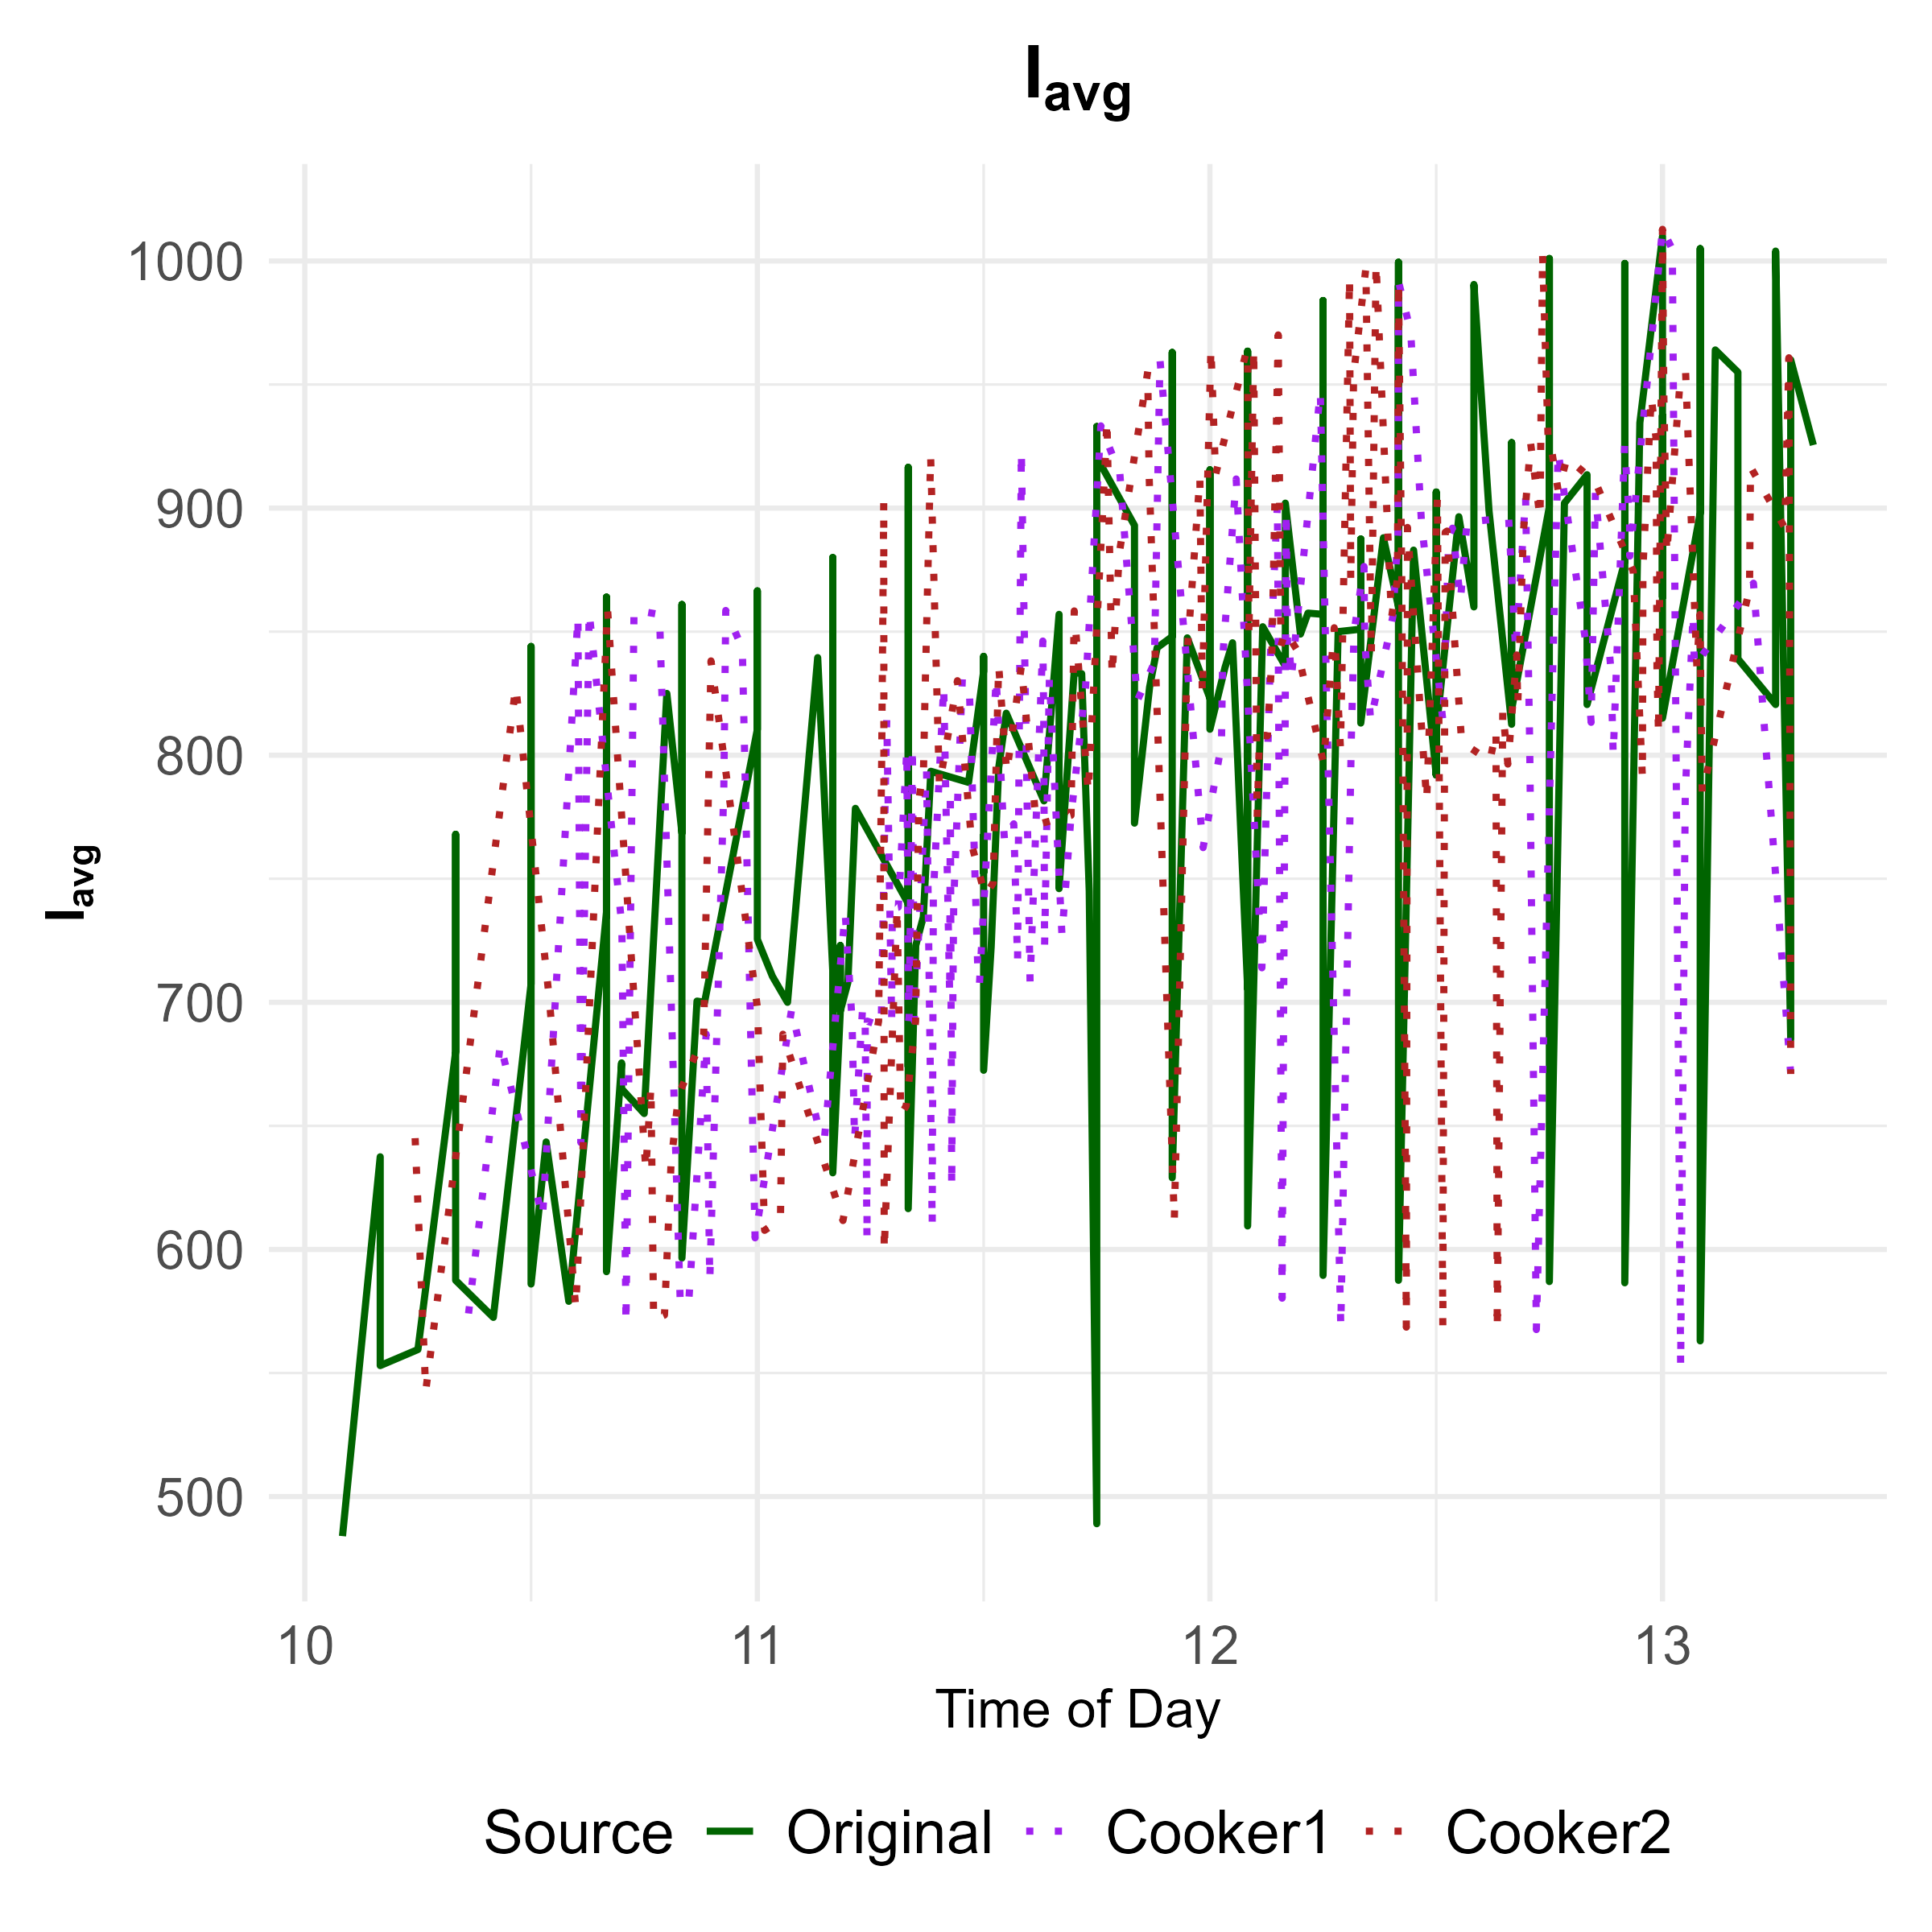
\includegraphics[width=0.8\textwidth, height= 10cm]{plots/ggplot_orig_vs_sim.png}
  \label{fig:Environmental_data_generation}
\end{figure}

\begin{algorithm}[H]
\caption{Baseline Survival Generator (Survfit Version)}
\label{alg:baseline-surv-survfit}
\SetAlgoLined
\KwIn{
  Reference level \(c^\ast\), covariate matrix \(X\),\\
  sample size \(n\), grid size \(N\), seed (opt.), flag \(p\)
}
\KwOut{
  Cox fit \(\hat\beta\), full grid \(\{t_j,H_0,S_0,F_0,f_0,\lambda_0\}\),\\
  sampled grid \(\{t_{k},H_0,S_0,F_0,f_0,\lambda_0\}\)
}
\BlankLine
\; Fit Cox model: \(\hat\beta = \arg\max_\beta \ell(\beta;X)\)\;
\; Extract baseline survival via \(\{(t_j,\hat S_0(t_j))\}\leftarrow\mathrm{survfit}()\) and set 
  \(\hat H_0(t_j)=-\log\hat S_0(t_j)\)\;
\; Interpolate \(\tilde H_0(t)\) by right‐continuous step or monotonic spline\;
\; Define grid: \(t_j = \mathrm{seq}(\min t,\max t,N)\)\;
\; Compute on grid:
  \[
    H_0(t_j)=\tilde H_0(t_j),\quad
    \lambda_0(t_j)=\frac{d}{dt}\tilde H_0(t),\quad
    S_0=e^{-H_0},\quad
    F_0=1-S_0,\quad
    f_0=S_0\,\lambda_0
  \]\;
\If{seed given}{\;\(\texttt{set.seed}(\cdot)\)\;}
\; Sample indices \(\{k_1,\dots,k_n\}\subset\{1,\dots,N\}\)\;
\; Extract \(\{t_k,H_0,\lambda_0,S_0,F_0,f_0\}\) at sampled \(t_k\)\;
\If{\(p\)}{\;Plot curves and sampled points\;}
\; \Return \(\hat\beta,\) full and sampled grids
\end{algorithm}

\begin{figure}[H]
  \centering
  \includegraphics[width=0.8\textwidth, height= 10cm]{plots/baseline_hazard_plot.png}
  \label{fig:baseline-cumhaz}
\end{figure}

\begin{algorithm}[H]
\DontPrintSemicolon
\SetAlgoLined
\SetKwInOut{Input}{Input}
\SetKwInOut{Output}{Output}

\Input{
  $\hat\beta$: estimated Cox coefficients,\\
  $(t_j,H_0(t_j))_{j=1}^m$: Breslow baseline hazard grid,\\
  $\{x_i\}_{i=1}^n$: covariate vectors,\\
  $C$: administrative censoring time.
}
\Output{
  $\{(\tilde T_i,\Delta_i)\}_{i=1}^n$: simulated times and event indicators.
}

\For{$i\leftarrow 1$ \KwTo $n$}{
  $\eta_i \leftarrow x_i^\top \hat\beta$\;
  Draw $U_i \sim \mathrm{Uniform}(0,1)$\;
  $y_i \leftarrow -\ln(U_i)\,/\,\exp(\eta_i)$\;
  \tcp*{Invert Breslow step‐function}
  $j^* \leftarrow \min\{\,j : H_0(t_j)\ge y_i\}$\;
  \eIf{$j^*$ exists}{
    $T_i \leftarrow t_{j^*}$\;
  }{
    $T_i \leftarrow +\infty$\;
  }
  \tcp*{Right‐censor at $C$}
  $\tilde T_i \leftarrow \min(T_i,\,C)$\;
  $\Delta_i \leftarrow \mathbf{1}\{T_i \le C\}$\;
}
\Return $\{(\tilde T_i,\Delta_i)\}_{i=1}^n$\;
\caption{Semi‐parametric inverse‐transform simulation for Cox model}
\label{alg:breslow-sim}
\end{algorithm}

\begin{algorithm}[H]
\caption{Sample‐Size Estimation via Cox PH Simulation}
\label{alg:coxph-sim}
\SetAlgoLined
\KwIn{$\mathcal N=\{N_1,\dots,N_k\}$, OR, $\alpha$, $\pi_{\rm target}$, $B$, seed, $T_{\max}$, \texttt{include\_plastic\_bag}, \texttt{test\_type}}
\KwOut{$N^* = \min\{N\in\mathcal N:\,\hat\pi(N)\ge\pi_{\rm target}\}$}
set \texttt{seed}\;
\ForEach{$N\in\mathcal N$}{
  $p\leftarrow\emptyset$, \quad $n\leftarrow2N$, \quad $\beta\leftarrow\log(\mathrm{OR})$\;
  \For{$b=1$ \KwTo $B$}{
    simulate covariates $Z_i$ for $i=1,\dots,2N$\;
    $\eta_i \gets Z_i^\top\beta$\;
    \texttt{res} $\gets$ \texttt{generate\_baseline\_functions}(n)\;
    $S_0\gets\mathrm{res.surv}$\;
    $S_{t|Z_i} \gets S_0^{\exp(\eta_i)}$\;
    $\tilde T_i\gets\min(T_i,\,T_{\max})$,\quad $\delta_i\gets\mathbf1\{T_i\le T_{\max}\}$\;
    fit Cox PH on $(\tilde T,\delta,Z)$ → $p_b$\;
    \uIf{\texttt{test\_type} = "one-sided"}{
      $p_b \gets p_b / 2$ \tcp*[r]{adjust for one-sided test}
    }
    $p\gets p\cup\{p_b\}$\;
  }
  $\hat\pi(N)\gets\dfrac1B\sum_{p_b\in p}\mathbf1\{p_b<\alpha\}$\;
}
\Return $N^*$  
\end{algorithm}

\begin{algorithm}[H]
\caption{Sample Size Determination via LMM Power Simulation}\label{alg:power_sample_size}
\DontPrintSemicolon
\SetAlgoLined
\KwIn{Pilot data $\mathcal{D}$ with response $P_s$, covariates $V$, cluster ID \texttt{TestDate};\\
  sample‐size grid $\{n_k\}$; desired effect $\delta$; significance level $\alpha$; target power $1-\beta$;\\
  number of simulations $N_{\rm sim}$; noise scale $\sigma$; RE shift scale $\tau$; optional ICC}
\KwOut{Optimal sample size $n^*$; power curve $\{(n_k,\widehat\pi(n_k))\}$}

\BlankLine
\textbf{Step 1: Hypotheses}\;
Define the parameter of interest
\[
  \theta \;=\; \operatorname{E}[P_s \mid \text{new}] \;-\; \operatorname{E}[P_s \mid \text{ref}].
\]
Then
\[
  \begin{cases}
    H_0:\,\theta\le0,\quad H_1:\,\theta\ge\delta & \text{(one‐sided)}\\[6pt]
    H_0:\,\theta=0,\quad H_1:\,\theta\neq0      & \text{(two‐sided)}
  \end{cases}
\]

\BlankLine
\textbf{Step 2: Baseline model \& variance extraction}\;
Fit LMM on $\mathcal{D}$:
\[
  P_s \sim V + (1\mid\texttt{TestDate}),
\]
and extract $\widehat\sigma_b^2$ and $\widehat\sigma_e^2$.  
\If{ICC is provided}{
  \[
    \widehat\sigma_b^2 \;\gets\; \frac{\mathrm{ICC}}{1-\mathrm{ICC}}\;\widehat\sigma_e^2.
  \]
}

\BlankLine
\textbf{Step 3: Power simulation for each $n_k$}\;
\For{$n_k$ \KwTo\ $\{n_k\}$}{
  $r\gets0$\tcp*{rejection counter}
  \For{$i\gets1$ \KwTo\ $N_{\rm sim}$}{
    Generate covariates via \texttt{get\_spline\_df\_dup\_cookers}($n_k,\tau,\sigma$)\;
    Sample cluster IDs, draw $b_j\sim N(0,\sigma_b^2)$ and $\varepsilon\sim N(0,\sigma_e^2)$\;
    Compute baseline prediction $\hat f(V)$ (fixed effects only)\;
    Form outcomes:
    \[
      Y_{\text{ref}} = \hat f + b_j + \varepsilon,
      \quad
      Y_{\text{new}} = \hat f + \delta + b_j + \varepsilon.
    \]
    Label data by \texttt{Cooker}; fit
    \[
      P_s \sim \texttt{Cooker} + V + (1\mid\texttt{TestDate}).
    \]
    Extract $\hat\beta$, SE, and
    \eIf{\texttt{Pr(>|t|)} in output}{
      $p_{\rm raw}\gets$ model p‐value
    }{
      $t\gets\hat\beta/\mathrm{SE}$,\quad
      $\mathrm{df}\gets n_{\rm obs}-p$,\quad
      $p_{\rm raw}\gets 2\bigl(1 - F_{t}(|t|;\mathrm{df})\bigr)$
    }
    Adjust for one‐ or two‐sided: obtain $p_i$\;
    \If{$p_i<\alpha$}{$r\gets r+1$}
  }
  $\widehat\pi(n_k)\gets r/N_{\rm sim}$
}

\BlankLine
\textbf{Step 4: Select optimal $n^*$}\;
$n^*\gets\min\{n_k:\widehat\pi(n_k)\ge1-\beta\}$ (or NA if none)\;

\Return{$n^*$ and $\{(n_k,\widehat\pi(n_k))\}$}
\end{algorithm}

\end{document}
